\section{EXPERIMENTS}\label{results}

\subsection{Comparison with the Virtual Hitting Plane method}

In this section, we compare in simulation the ball returning performance of our new approach against the virtual hitting plane (VHP) method. The VHP method that we implement is a close variant of \cite{Muelling13}. In this approach, the specification of the VHP fixes the hitting time $\hitTime$ as well as the hitting point $\ballEst(\hitTime)$ for the racket trajectory. The remaining parameters, the desired racket velocity $\racketVel_{\mathrm{des}}(\hitTime)$ and the desired racket normal at hitting time $\normal_{\mathrm{des}}(\hitTime)$ are found by using the models~\eqref{flightModel} and \eqref{mirrorLaw}. First, a desired landing point $\ballLand$ and a desired time duration $\landTime$ are specified. A desired ball outgoing velocity is then found by solving the boundary value problem for the flight model~\eqref{flightModel} with the boundary values
%
\begin{align}
&\ball(\hitTime) = \ballEst(\hitTime), \\
&\ball(\landTime) = \ballLand.
\label{bvp}
\end{align}
%
Afterwards, $\racketVel_{\mathrm{des}}(\hitTime)$ and $\normal_{\mathrm{des}}(\hitTime)$ are calculated by inverting the reflection model~\eqref{mirrorLaw}. The inversion results in the desired racket velocity along the normal $v_n$ and the desired normal. Racket velocity along the other two directions are fixed to zero to minimize any accidental generation of spin.

To run inverse kinematics (IK) on the desired hitting point, one needs to additionally specify a desired racket slide~\cite{Spong06}. An easy and convenient way to generate a desired racket slide at hitting time is to rotate the initial racket slide until the initial racket normal aligns with the final desired racket normal. This procedure determines the full orientation of the final robot posture at hitting time, running IK then will specify the final joint positions. To make IK more robust, we provide initial estimates from a lookup table. We look up the Cartesian and joint position values reached at the striking time estimates \eqref{strikingTimeEst} during our demonstrations. We can perform linear regression or interpolate between this demonstration data to quickly come up with good initial estimates.
%by a human holding the Barrett WAM arm during kinesthetic teach-in. 

Final joint velocities are found after running IK by using the Jacobian at hitting time and the desired racket velocities as in~\eqref{transCond2}. After generating a third degree polynomial in joint space, we check for joint limitations, and the Cartesian constraints due to the table. The actual joint limits for the Barrett WAM are shown in Table~\ref{joint limits} in the appendix. 

When the ball is coming close to the robots initial posture, this complicated procedure results in feasible trajectories if the VHP is chosen appropriately. However, it is very inflexible and the IK procedure can easily fail to find good configurations. 

To make a fair comparison between the VHP approach and our algorithm $\alg$, in our simulation environment\footnote{Code for our simulation platform is available in our git repository: https://github.com/RobotLearning/traj-gen-and-tracking.git} we fix the initial ball state variance such that most balls end up close to the initial robot posture. This ensures that we make a fair evaluation between the two algorithms. Both methods filter the incoming stream of ball position estimates with the same EKF and equally predict the time to pass over the table $T_{\mathrm{table}}$. If this value is less than $T_{\mathrm{max}} = 0.6$ sec, trajectory generation is launched. This occurs generally after the ball passes the net.

\begin{table}
\renewcommand{\arraystretch}{1.3}
\caption{Simulation results comparing $\alg$ and VHP-method}
\label{tableSimResults}
\centering
\begin{tabular}{c||c|c|c|c}
& \bfseries Returns & \bfseries Not Valid  & \bfseries Limits Violated & \bfseries Missed/Outside \\
\hline
$\alg$ & 151 & 24 & 19 & 6\\
\hline
VHP & 125 & 24 & 45 & 6\\
\hline
\end{tabular}
\end{table}
%
\begin{figure}[t!]
\centering
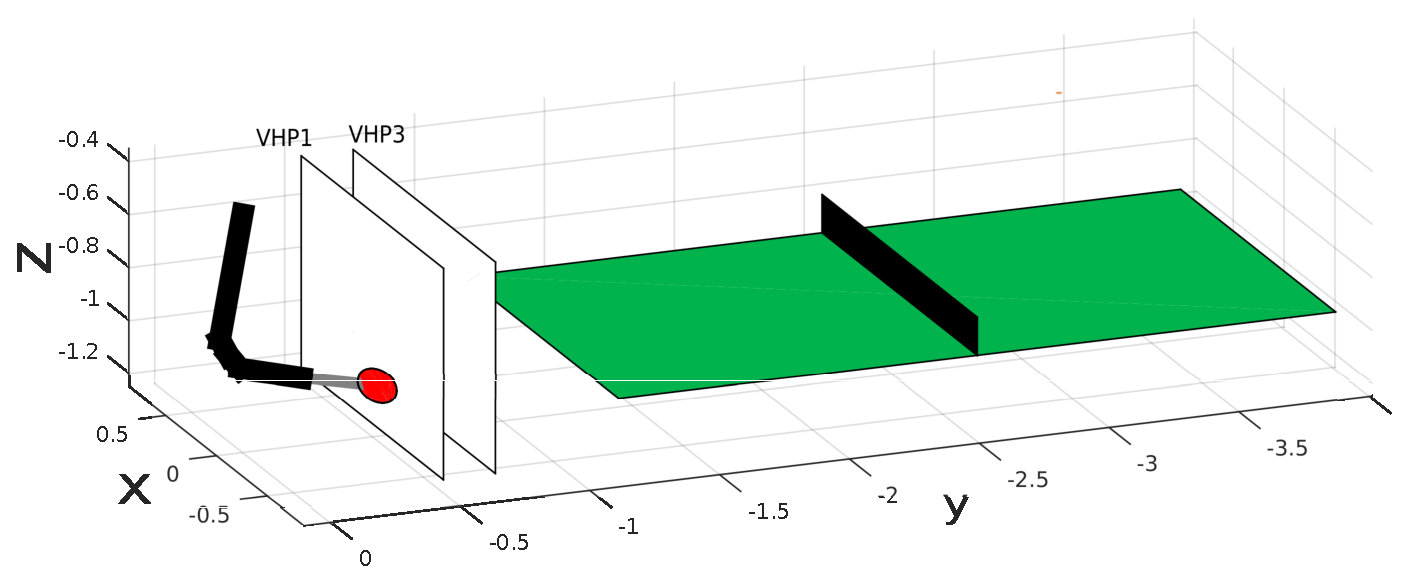
\includegraphics[scale=0.25]{tableTennisVHP.eps}			
\caption{For simulating the performance of the VHP method in a fair way, we average the results over four different VHP locations. The first and third plane locations are shown in the figure. Out of $50$ balls each, the VHP methods with $y = -0.7,-0.6,-0.5,-0.4$ return $31, 37, 28, 29$ balls respectively.}
\label{vhps}
\end{figure}
%
We summarize our evaluations in Table~\ref{tableSimResults}. A total of $200$ balls are launched towards the robot in single-ball solo trials from varying initial positions and velocities. The initial ball mean $\vec{\mu}_{\mathrm{init}}$ is fixed at a sensible value and the initial covariance matrix is diagonal with a standard deviation of $\sigma_{\mathrm{init}} = 0.1$, i.e. $\ball_{\mathrm{init}} \sim \mathcal{N}(\vec{\mu}_{\mathrm{init}}, \vec{\Sigma}_{\mathrm{init}})$, $\vec{\Sigma}_{\mathrm{init}} = \sigma_{\mathrm{init}}^2 \vec{I}$. Some balls are illegal, for example they might not bounce on the robot's court. Such balls are detected with our ball prediction models and they are not considered for strike generation. They are marked as \emph{Not Valid} in Table~\ref{tableSimResults}. The attached video shows example solo trials in our simulation platform with both methods.

Comparing with the VHP method, we see that $\alg$ is able to return more balls to the other side, with $26$ more balls returned to the opponent's court. One of the main reasons for this increase in performance is the fixed location of the VHP. Depending on the incoming ball velocity, trajectories generated using a fixed VHP can result in joint limit violations or infeasible solutions. They are marked as \emph{Limits Violated} in Table~\ref{tableSimResults}. A second reason is the explicit incorporation of joint limits both for the striking trajectory and the return trajectory in our optimization problem. See Figure~\ref{vhps} for an illustration. Out of $50$ balls each, the VHP methods with the planes fixed at $y = -0.7,-0.6,-0.5,-0.4$ locations return $31, 37, 28, 29$ balls respectively. For this particular ball distribution, the plane at $y = -0.7$ seems to be the most robust option.
% talk more on the GP models
% figure needed

% Shall we put a small video for simulations?

\subsection{Discussion}

\begin{figure}
  \begin{subfigure}[b]{0.45\textwidth}
    \centering
    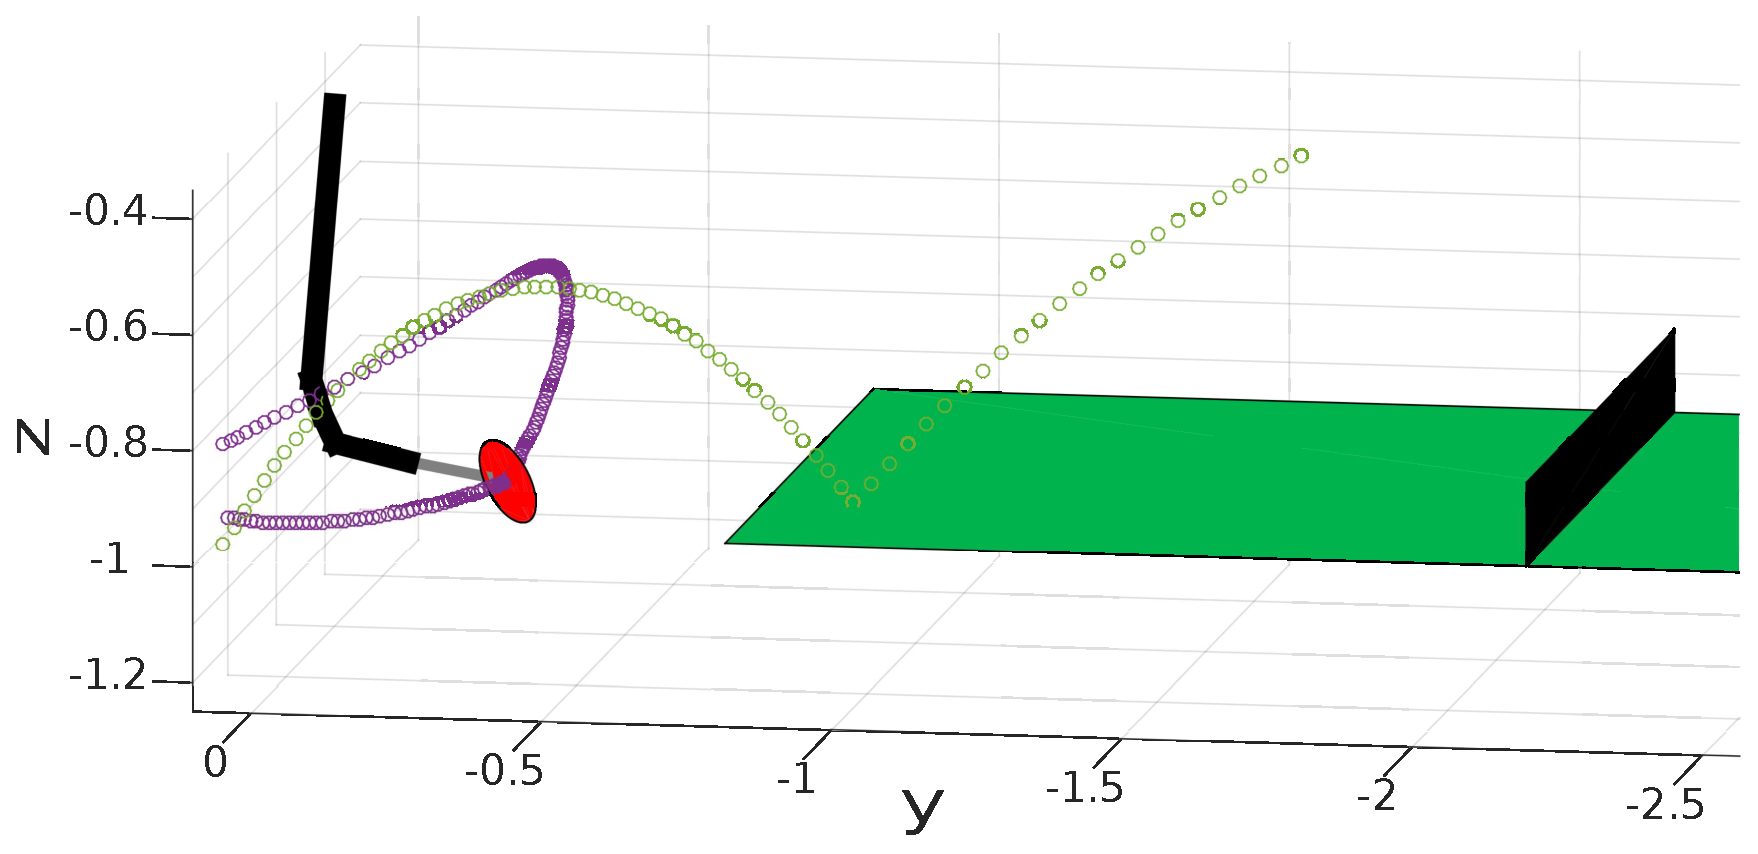
\includegraphics[width=\textwidth]{racket_ball_traj_0.eps}
    \caption{Rest posture}
    \label{fig:1}
  \end{subfigure}
  
  \begin{subfigure}[b]{0.45\textwidth}
  	\centering
    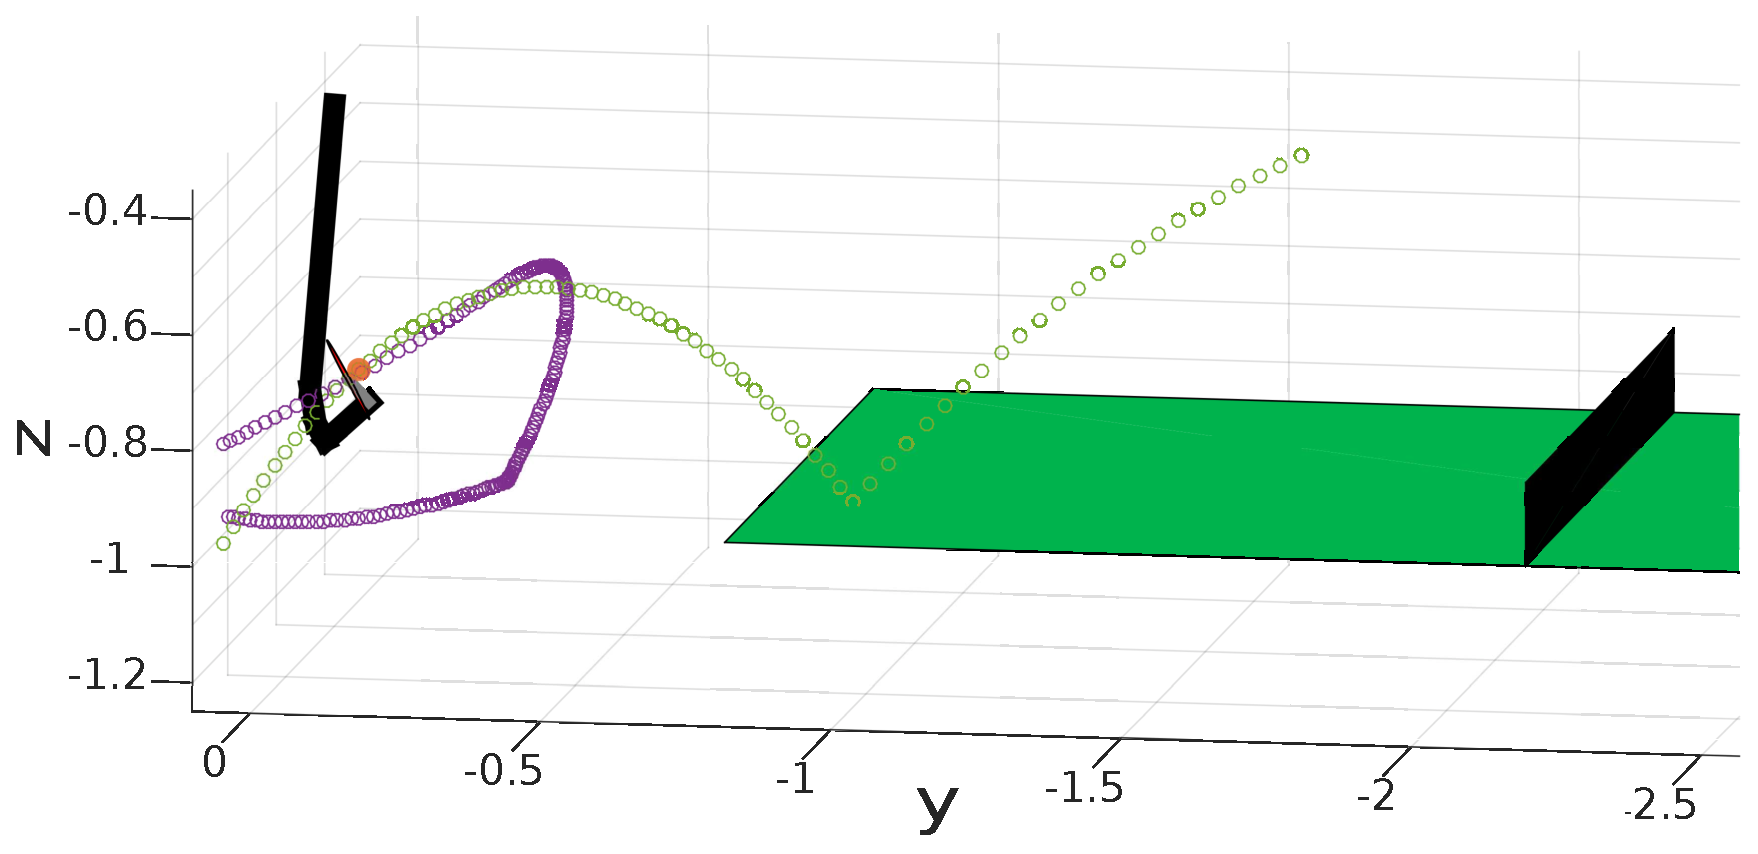
\includegraphics[width=\textwidth]{racket_ball_traj_1.eps}
    \caption{Posture at striking time}
    \label{fig:2}
  \end{subfigure}
  \caption{An example trajectory generated by our optimal control based framework. The resulting trajectory, minimizing the accelerations throughout, incorporates naturally a swingback pattern that may not be included in other methods fixing a virtual hitting plane (VHP).}
  \label{fig:0}
\end{figure}

\begin{figure}[t!]
\centering
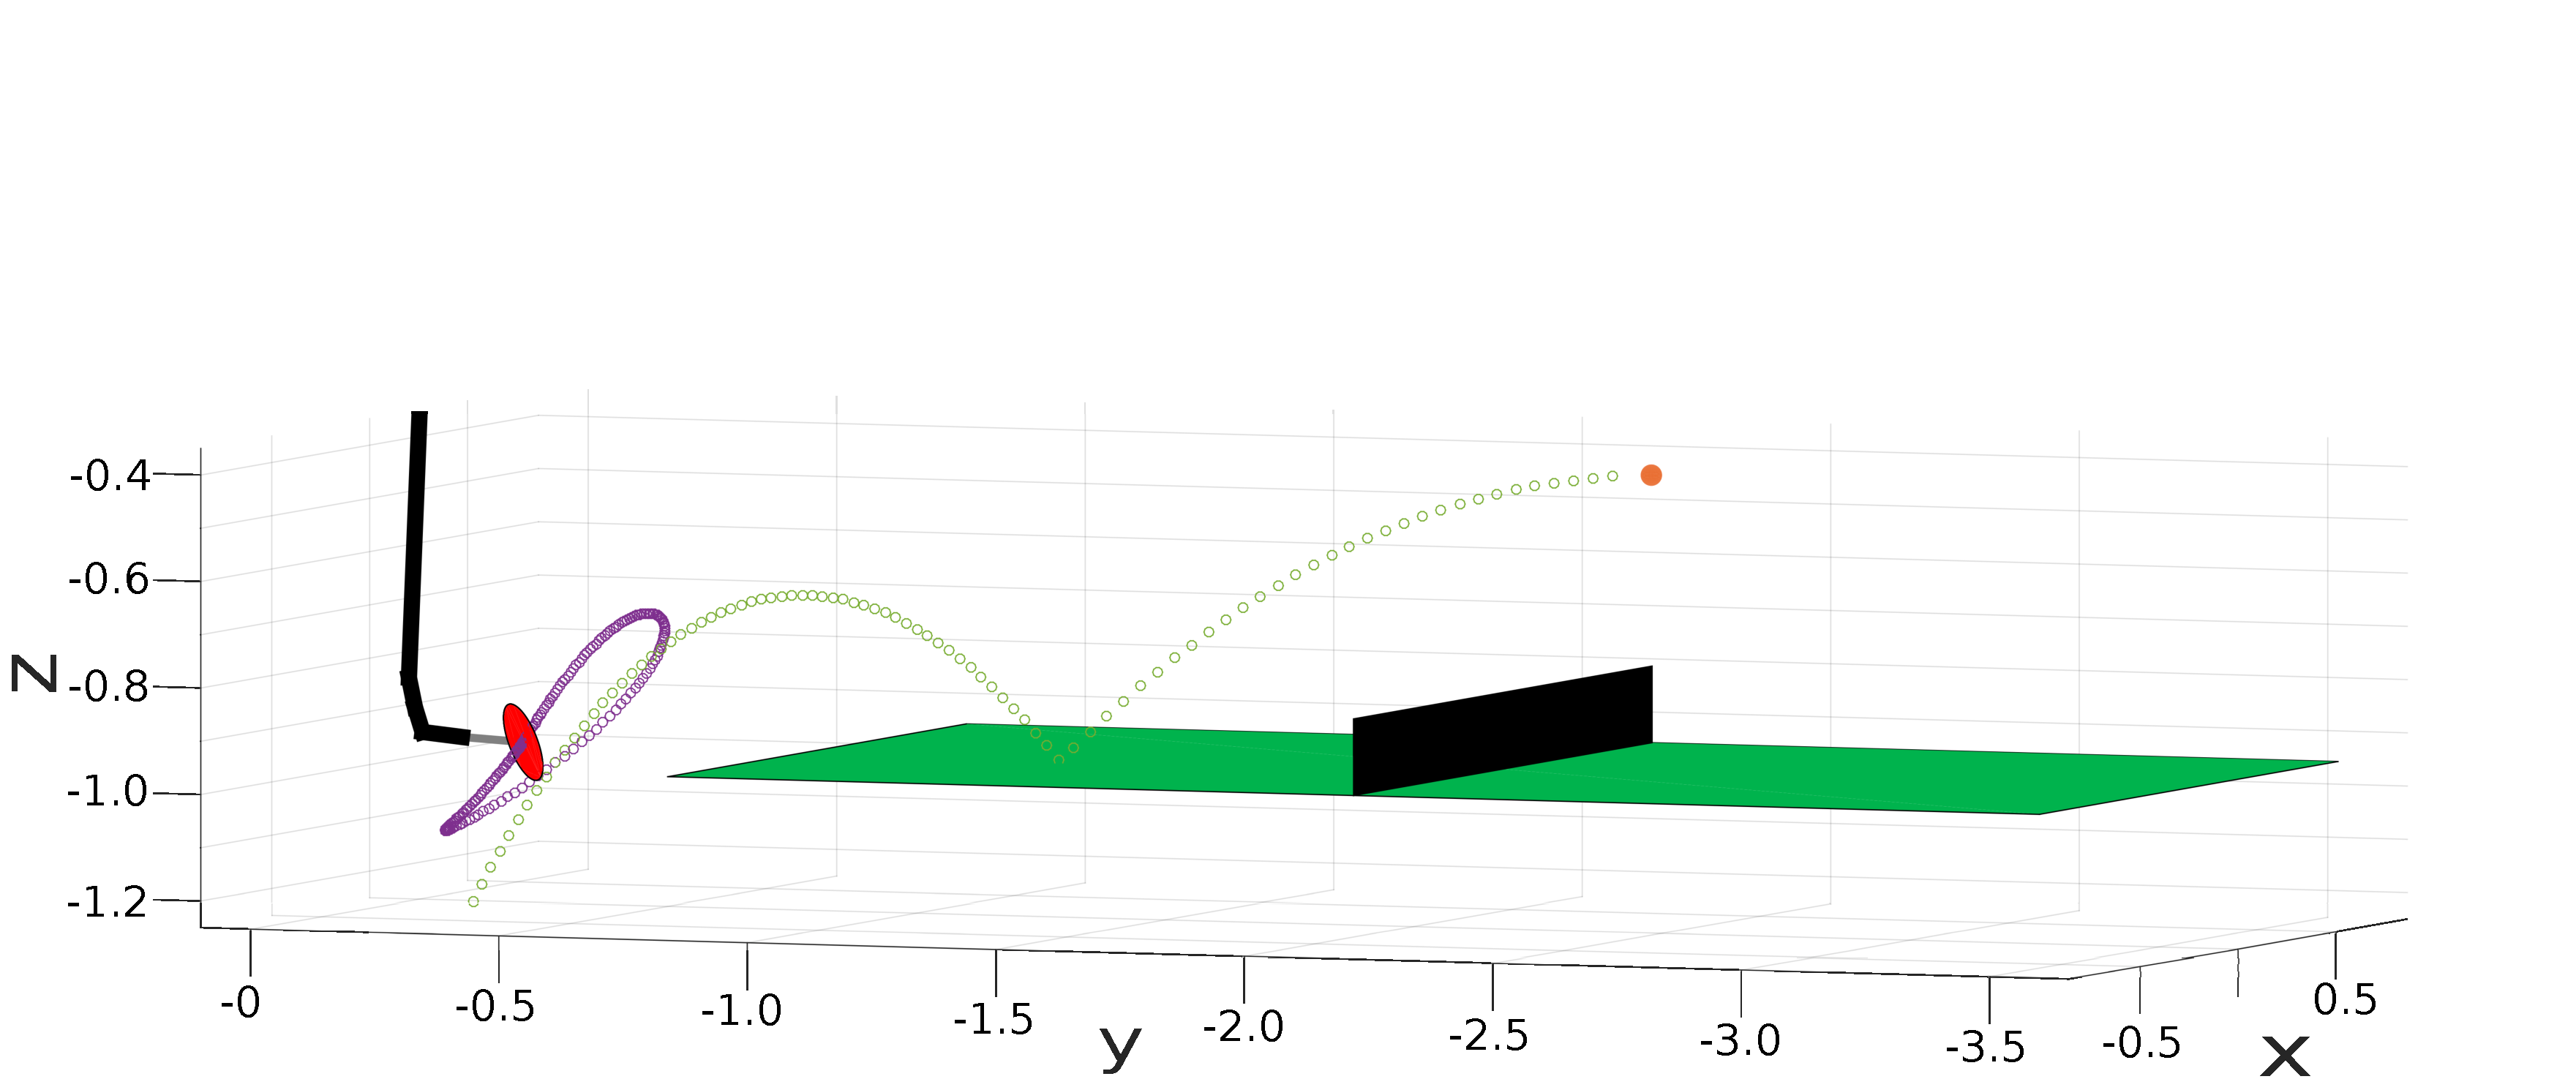
\includegraphics[scale=0.15]{racket_ball_traj_2.eps}	
\caption{Another computed optimal trajectory. In this case, there is less swingback and the alignment with the ball trajectory is higher.}
\label{fig:3}
\end{figure}

Two example Cartesian trajectories computed by our method are shown in Figure~\ref{fig:0} and Figure~\ref{fig:3}. The figures are snapshots of our realistic simulation platform. Resulting trajectories naturally incorporate a swingback motion whenever needed, without explicit programming. More natural strikes can be computed in our framework. In the case shown in Figure~\ref{fig:0} for example, setting a VHP in front of the robot would result in very high accelerations, whereas the computed optimal trajectory intercepts with the ball trajectory behind the initial pose of the robot.

The realistic simulation platform is designed to imitate the features of our robotic table tennis setup, see Figure~\ref{robot}. All the specifications in the robotic the same as in our simulation environment. Our robot is a seven degree of freedom custom-made Barrett WAM arm that can easily reach $10g$ m/$\textrm{s}^2$ accelerations. It is torque-controlled and cable-driven. A standard size racket ($8$ cm radius) is attached to the end-effector. Our vision system tracks the balls at a rate of $60$ Hz and consists of four cameras on the corners on the ceiling. See~\cite{Lampert12} for platform details. Each camera provides raw blob data which is first fused together and then filtered with an Extended Kalman Filter (EKF). The table and the tennis balls are standard sized, the balls have a radius of $2$ cm, the table geometry is approximately $276 \times 152 \times 76$ cm.

In our robot experiments we can use a ball-launcher (see Figure~\ref{robot}) to throw balls to the right hand side of the robot. The ball generally comes with a high variance, especially the velocities are quite unpredictable even without oscillating the ball-launcher. The robot is at a distance of roughly $115$ cm. The robot's forehand posture $\joint_0$ can be chosen the same as in our simulations. We think that the new trajectory generation framework offers a promising solution for robotic table tennis. 

\begin{figure}[t!]
\centering
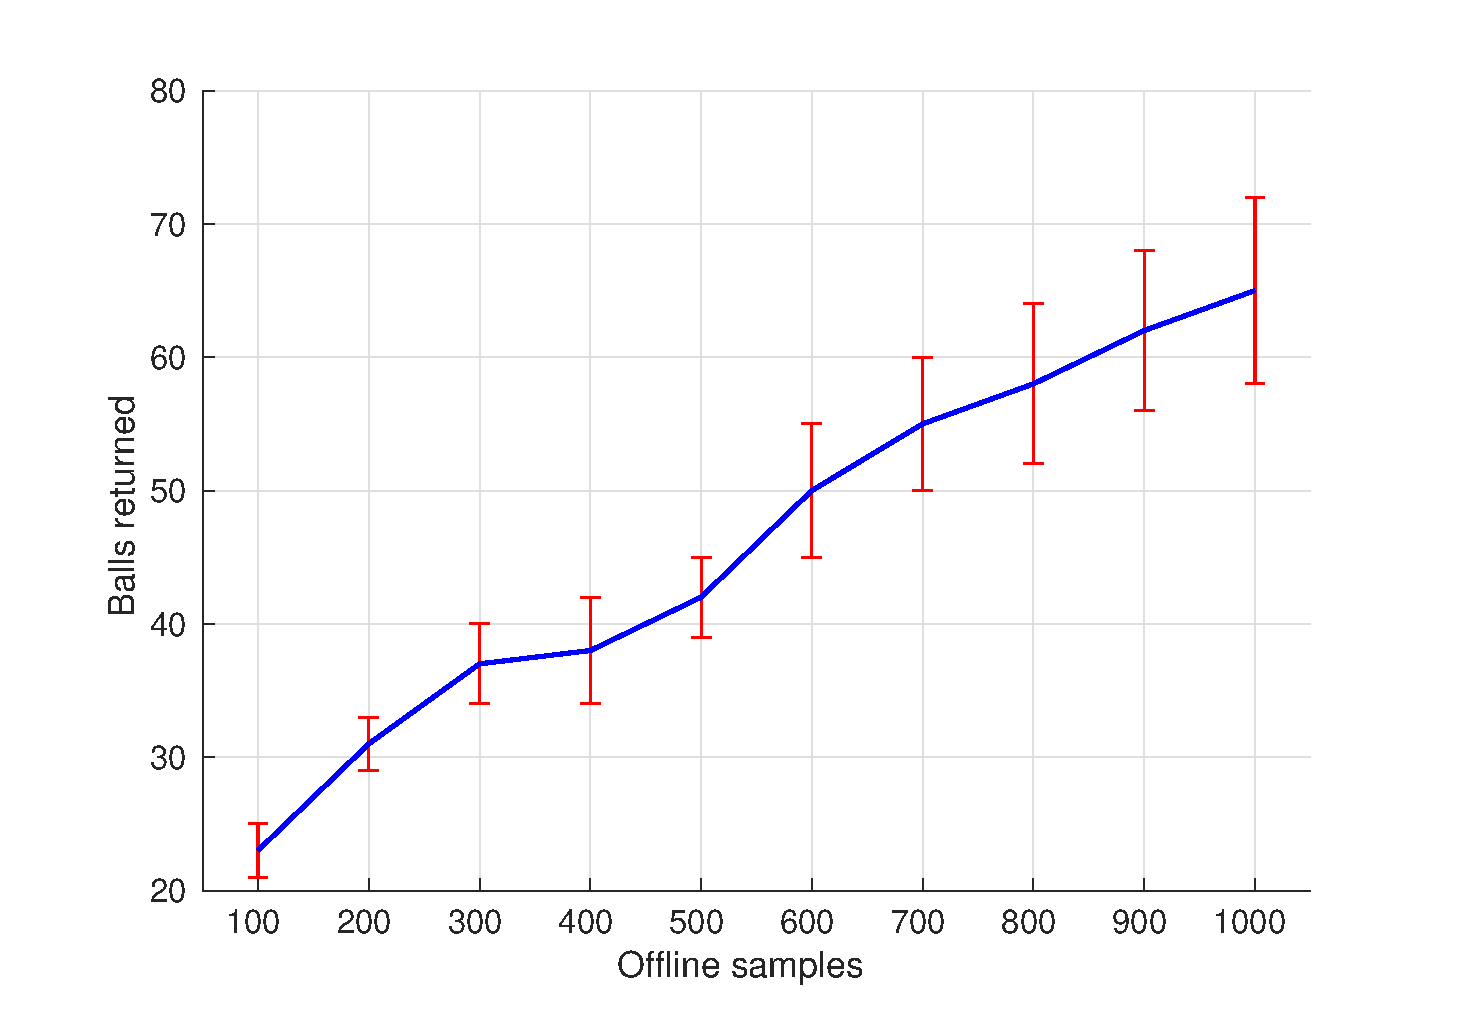
\includegraphics[scale=0.30]{offline.eps}	
\caption{Performance of our trajectory generation framework using a lookup table constructed offline. Results are averaged over $5$ different runs. As the number of stored lookup table samples increase, the performance approaches that of the online trajectory generation. One should bear in mind that illegal balls (12-13 \% on average) are counted as unsuccessful trials.}
\label{fig:offline}
\end{figure}

Unfortunately, our optimization takes currently about two seconds on our system on average. One of the ways to show its performance in the table tennis setup is to use a lookup table. In Figure~\ref{fig:offline} we evaluate the performance of the lookup table, measured in terms of the percentage of incoming balls returned successfully to the opponent's court. The same initial ball distribution with the same $\vec{\mu}_{\mathrm{init}}, \vec{\Sigma}_{\mathrm{init}}$ values is used as before. Whenever a strike is successful in returning the ball in simulation offline, we store in the lookup table ball positions, velocities at the start of the movement, i.e. $T_{\mathrm{table}} < T_{\mathrm{max}}$, and the optimized parameters $\joint_f, \dot{\joint}_f, T$. We can then at runtime simply lookup the optimized parameters that have the closest stored ball position and velocity estimates. As the number of lookup table samples increase, the performance in simulation approaches that of the online trajectory generation. We already incorporate the estimated parameters of our physical models in our offline computations, hence we expect that the lookup table with sufficient sample size will be able to play table tennis in our robotic setup. See Figure~\ref{fig:rebound} for rebound model estimation results.

% vision system operates in a semi-structured and human-inhabited environment
% Finite State Automaton: four stages: awaiting stage, preparation, hitting and finishing stage